\documentclass[a4paper]{article}

\usepackage[english]{babel}
\usepackage[utf8]{inputenc}
\usepackage{amsmath}
\usepackage{graphicx}
\usepackage[colorinlistoftodos]{todonotes}

\usepackage{theorem}
\usepackage{amssymb}

\usepackage{hyperref}

\usepackage{caption}
\usepackage{subcaption}

\newenvironment{proof}{{\bf Proof:  }}{\hfill\rule{2mm}{2mm}}

\newtheorem{fact}{Fact}[section]
\newtheorem{lemma}[fact]{Lemma}
\newtheorem{theorem}[fact]{Theorem}
\newtheorem{definition}[fact]{Definition}
\newtheorem{corollary}[fact]{Corollary}
\newtheorem{proposition}[fact]{Proposition}
\newtheorem{claim}[fact]{Claim}
\newtheorem{exercise}[fact]{Exercise}

\usepackage{algorithm}
\usepackage{algorithmic}

\makeatletter
\newcommand{\distas}[1]{\mathbin{\overset{#1}{\kern\z@\sim}}}%
\newsavebox{\mybox}\newsavebox{\mysim}
\newcommand{\distras}[1]{%
  \savebox{\mybox}{\hbox{\kern3pt$\scriptstyle#1$\kern3pt}}%
  \savebox{\mysim}{\hbox{$\sim$}}%
  \mathbin{\overset{#1}{\kern\z@\resizebox{\wd\mybox}{\ht\mysim}{$\sim$}}}%
}
\makeatother

\newcommand{\RT}[1]{\marginpar{\footnotesize\color{red}RT: #1}}

\title{Law of Large Graphs}

\date{\today}

\begin{document}
\maketitle

\section{Introduction}

Mean is one of the most important and basic concept in statistics. Motivated by the law of large numbers, sample mean is always considered to be the best estimate of the population mean. Nowadays we take averages almost everywhere, from the fundamental elements in Euclidean space to more general objects, like shapes, documents and graphs.

However, contradicting to the general intuition, arithmetic average should not be our first choice all the time. In 1955, Stein's paradox \cite{efron1977stein} shows the inadmissibility of the sample mean when there are more than three normal distributions. The fact that James-Stein estimator dominates the sample mean makes it less preferable to take the average in that situation. 27 years later, Gutmann proved that this cannot occur when the sample spaces are finite \cite{gutmann1982stein}. But even when sample mean is admissible, it doesn't close the door of other estimators to be better in some cases. So in a specific situation, for instance a collection of graphs considered in this paper, there is always a chance to have a better estimator compared to the sample mean.

Before introducing the new estimator other than the sample mean for graphs, we need to know what the mean of a collection of graphs is. Although it can be defined in various ways, we pick the natural definition as the proportions of the existence of an edge between any pair of vertices. Estimating the mean of a population of graphs based on a sample is becoming more and more important both in statistical inference and in various applications like connectomics, social networks, etc.

Element-wise maximum likelihood estimate (MLE), which happens to be the sample mean in many situations, is a reasonable estimator if we only consider the independent edge model (IEM) \cite{bollobas2007phase} without taking any graph structure into account. However, it does not perform very well especially when only a few observations are available, which happens a lot in practice.

Intuitively, an estimator incorporating the graph structure is preferable than the entry-wise MLE. But we don't have any knowledge about the structure of the graphs in general. So it is hard to take advantage of the unknown graph structure.

One of the most important structures is the community structure in which vertices are clustered into different communities and the ones of the same community behave similarly. The stochastic blockmodel (SBM) \cite{holland1983stochastic} captures such structural property and is widely used in modeling networks.

Meanwhile, the latent positions model (LPM) \cite{hoff2002latent}, a much more general model compared to SBM, proposes a way to parameterize the graph structure by latent positions associated with each vertex. The random dot product graph (RDPG) \cite{young2007random, nickel2007random} which is a special case of LPM stays in between and motivates our estimator. In this paper, we analyze our estimator in terms of RDPG specifically.

Using the estimates of the latent positions in an RDPG setting based on a truncated eigen-decomposition of the adjacency matrix, we consider a new estimator for the mean of the collection of graphs which captures the low-rank structure. In this study, we prove via theory, simulations and real data analysis that it is better than element-wise MLE.

Nowadays, people care about information that can be extracted from the networks through different ways in neuroscience.
For instance, Ginestet et al. \cite{ginestet2014hypothesis} proposed a way to test if there is a difference between the networks of two groups of subjects. While hypothesis testing is the final goal, estimation as a stepping stone could be improved by our method. Thus the estimator in this study is not only useful in estimation, but also can be applied to help improve other statistical inferences.

(Future work) Robust estimation, dimension selection, diagonal augmentation, etc.



\section{Models and Estimators}
\label{section:model_estimator}
This work considers the scenario of having $M$ graphs represented as adjacency matrices, $\{A^{(m)}\}$ ($m = 1, \cdots, M$), each having $N$ vertices with known correspondence. The graphs we consider are undirected and unweighted with no self-loops, i.e. each $A^{(m)}$ is a binary symmetric matrix with zeros along the diagonal. An example application of this arises in the field of connectomics, where functional brain imaging data for each subject can be represented as a graph, with each vertex having a defined anatomical correspondence, and an edge between two regions is defined to exist if correlation in activity between the regions reaches a certain threshold.



\subsection{Independent Edge Model}
The first basic model we consider is the independent edge model (IEM) with parameter $P \in [0,1]^{N\times N}$\cite{bollobas2007phase}, where each edge between vertex $i$ and vertex $j$ exists with probability $P_{ij}$ independently of all other edges. In this case, we aim to estimate the mean, i.e. probability matrix $P$, with our observations of the adjacency matrices $\{A^{(m)}\}$ of $M$ graphs.



\subsection{Estimator $\bar{A}$}
Under the IEM, element-wise sample mean of the adjacency matrices $\bar{A}$ is the MLE as well as the least squared estimate for $P$. It is unbiased with entry-wise variance $\mathrm{Var}(\bar{A}_{ij}) = P_{ij} (1-P_{ij})/M$. Moreover, $\bar{A}$ is the uniformly minimum-variance unbiased estimator (UMVUE), i.e. it has the smallest variance among all unbiased estimators.

However, $\bar{A}$ doesn't exploit any graph structure, and sometimes the performance is not very good especially when $M$ is small. For example, when $M=1$, $\bar{A}$ is exactly the binary graph we observe, which is an inaccurate estimate for an arbitrary $P$.



\subsection{Random Dot Product Graph}
In graphs, the adjacencies always depends on the unobserved properties of the corresponding vertices. For example, in a connectomics setting, the two brain regions with similar (some properties?) will have stronger connections.
The latent positions graph model (LPG) proposed by Hoff et. al. (2002) \cite{hoff2002latent} captures such structure. where each vertex is associated with a latent positions that influences the adjacencies for that vertex.
In this model, each vertex $i$ has an associated latent vector $X_i \in \mathbb{R}^d$ sampled from distribution $\mathcal{F}$. Based on those latent positions, the existence of edges are conditionally independent with probability only depends on the latent vectors of the incident vertices through a link function. Generally $d$ is much smaller than the number of vertices $N$, so it is a much more succinct model compared to IEM.

A specific instance of the LPG that we examine in this work is the random dot product graph model (RDPG) \cite{young2007random, nickel2007random} where the link function is the dot product, i.e. the probability of an edge being present between two nodes is the dot product of their latent vectors.

Formally, let $\mathcal{X} \subset \mathbb{R}^d$ be a set such that $x, y \in \mathcal{X}$ implies $\left \langle  x,y \right \rangle \in [0, 1]$, let $X_i\distas{iid} F$ on $\mathcal{X}$, and write $X = [X_1|\cdots|X_N]^T \in \mathbb{R}^{N \times d}$.
A random graph $G$ with adjacency matrix $A$ is said to be an RDPG if
\[
	P(A|X) = \prod_{i<j} \left \langle X_i, X_j \right \rangle^{A_{ij}} \left( 1 - \left \langle X_i, X_j \right \rangle \right)^{1 - A_{ij}}.
\]
In the RDPG model,each vertex $i$ is associated with a latent position $X_i$. Conditioned on the latent positions $X$, the edges $A_{ij} \distas{iid} \text{Bern}(\left \langle X_i, X_j \right \rangle)$.
Note that the probability matrix is the out product of the latent positions, i.e. $P = X X^T$.
%Note that $\mathrm{rank}(P) = \mathrm{rank}(X)$.




\subsection{Estimator $\hat{P}$ Based on Adjacency Spectral Embedding}

Motivated by the RDPG, we consider a new estimator $\hat{P}$ based on the adjacency spectral embedding (ASE) which enforce a low rank approximation on the entry-wise sample mean $\bar{A}$.

Since the graphs are symmetric, we can get $\hat{U} \hat{S} \hat{U}^T$ as the eigen-decomposition of $\bar{A}$, where $\hat{S}$ is a diagonal matrix with non-increasing entries along the diagonal. Then the $d$-dimensional ASE of $\bar{A}$ is the first $d$ columns of $\hat{U} |\hat{S}|^{1/2}$, denoted by $\hat{X} \in \mathbb{R}^{N \times d}$. The rows of $\hat{X}$ represent the estimated latent vectors for each vertex. 
Based on the low rank approximated RDPG representation of the sample mean matrix constructed by ASE, we define our new estimator as $\hat{P} = \hat{X} \hat{X}^T$.

To get $\hat{P}$, we need to specify what dimension $d$ that ASE uses. There are varies ways dealing with dimension selection. In this paper, we consider Zhu and Ghodsi's elbow selection method \cite{zhu2006automatic} and the universal singular value thresholding (USVT) method \cite{chatterjee2015matrix}. Details are discussed in Section \ref{section:dim_select}.

Moreover, since the graphs are hollow, i.e. with zeros along the diagonal, applying ASE directly will lead to a bias in calculating the eigenvalues. To compensate such bias, we use an iterative method developed by Scheinerman and Tucker \cite{scheinerman2010modeling}. Details are discussed in Section \ref{section:diag_aug}.


\begin{algorithm}[H]
\caption{}
\label{algo:basic}
\begin{algorithmic}[1]
\STATE \textbf{Input:} $A^{(1)}, A^{(2)}, \cdots, A^{(M)}$, each $A^{(m)} \in \{0,1\}^{N \times N}$ is symmetric and hollow, with known vertex correspondence;
\STATE Calculate the sample mean graph $\bar{A} = \frac{1}{M}\sum\limits_{m = 1}^M A^{(m)}$;
\STATE Augmented the diagonal of $\bar{A}$ to get $\bar{A} + D$ (see Section \ref{section:diag_aug});
\STATE Select the dimension $d$ to which we are going to embed $\bar{A} + D$ (see Section \ref{section:dim_select});
\STATE Calculate the eigen-decomposition, $\bar{A} + D = \hat{U} \hat{S} \hat{U}^T$;
\STATE Obtain $d$-dimensional ASE $\hat{X} \in \mathbb{R}^{N \times d}$ by the first $d$ columns of $\hat{U} |\hat{S}|^{1/2}$;
\STATE $\hat{P} = \hat{X} \hat{X}^{T}$ is our estimator.
\end{algorithmic}
\end{algorithm}



In order to take advantage of the underlying low rank structure of the RDPG, we use the adjacency spectral embedding (ASE) studied by Sussman et. al. to enforce a low rank approximation on the entry-wise mean matrix $\bar{A}$, which will decrease the variance without losing much in bias if we embed it into the right dimension.

\subsection{Stochastic Block Model as an Random Dot Product Graph}
\label{section:sbm_rdpg}
One of the most important structures is the community structure in which vertices are clustered into different communities such that vertices of the same community behave similarly. Such structural property is captured by the stochastic blockmodel (SBM) \cite{holland1983stochastic}, where each vertex is assigned to a block and the probability that an edge exists between two vertices depends only on their respective block memberships.

Formally, the SBM is parameterized by the number of blocks $K$ (generally way less than the number of vertices $N$), block probability matrix $B \in [0,1]^{K \times K}$ and block proportion vector $\rho \in (0,1)^K$ with $\sum_{k=1}^K \rho_k = 1$. Let $\tau$ represent the block memberships, then for any $i \in [n]$ and $k \in [K]$, $\tau(i) = k$ means vertex $i$ is assigned to block $k$. And each vertex is assigned independently with probability vector $\rho$, i.e. $P(\tau(i) = k) = \rho_k$. Conditioned on $\tau$, each entry of the adjacency matrix $A_{ij}$ is independently sampled from the Bernoulli distribution with parameter $B_{\tau_i,\tau_j}$.

In order to analyze the estimator $\hat{P}$ motivated by RDPG, we move to another representation of SBM based on RDPG. Consider a positive semi-definite $K$-block SBM with a rank $d (\le K)$ block probability matrix $B$, we can always decompose $B$ into $\nu \nu^T$, where $\nu \in \mathbb{R}^{K \times d}$ and each row $\nu_k$ is the shared latent position for all vertices assigned to block $k$. Let $X \in \mathbb{R}^{N \times d}$ with each row to be $X_i = \nu_{\tau_i}$, then we have
\[
	P(A_{ij} = 1|\tau) = B_{\tau_i, \tau_j} = \nu_{\tau_i}^T \nu_{\tau_j}.
\]
Note that the SBM can be seen as an RDPG with $X_i \distas{iid} \sum_{k=1}^K \rho_k \delta_{\nu_k}$, i.e. all vertices in the same block will have identical latent positions.

To better illustrating what an SBM actually looks like, in Figure \ref{fig:SBM_example} we consider a 5-block SBM and plot the corresponding probability matrix and one adjacency matrix generated from it with 200 vertices. From the figure, we can clearly see the structure of 25 blocks in both the probability matrix and the adjacency matrix as a result of 5 different blocks among vertices.

\begin{figure}
\centering
\begin{subfigure}{.5\textwidth}
  \centering
  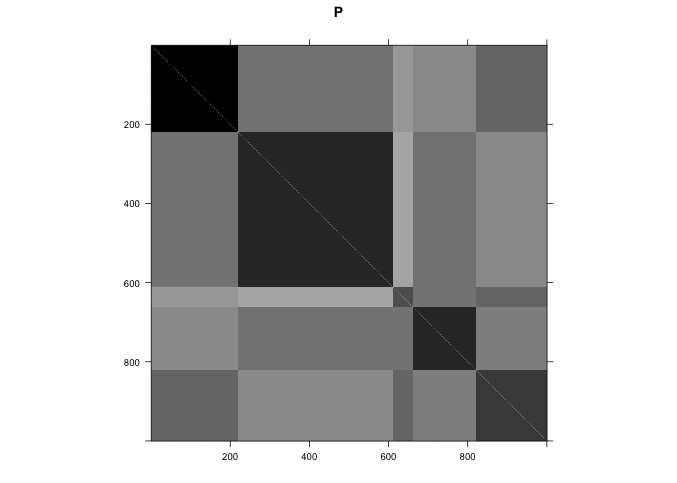
\includegraphics[width=1.2\linewidth]{SBM_P.png}
\end{subfigure}%
\begin{subfigure}{.5\textwidth}
  \centering
  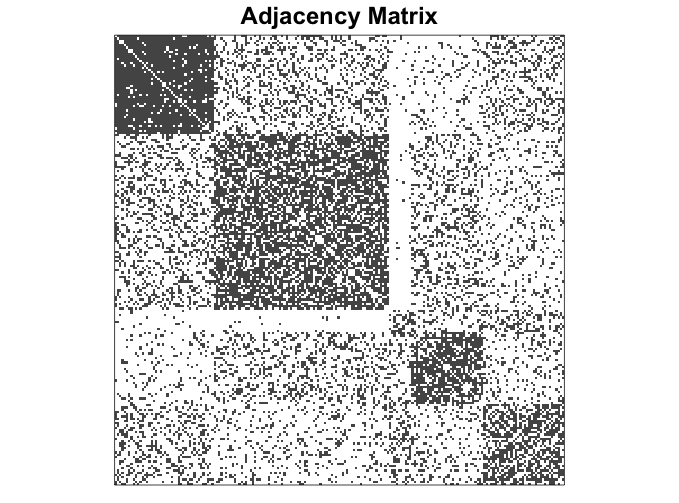
\includegraphics[width=1.2\linewidth]{SBM_A.png}
\end{subfigure}
\caption{Example illustrating the SBM. The figure on the left is the probability matrix $P$ that follows a SBM with $K = 5$ blocks; The other figure shows the adjacency matrix $A$ for 200 vertices generated from the SBM with probability matrix $P$.}
\label{fig:SBM_example}
\end{figure}



\section{Results}

\subsection{Theoretical Results}
\label{section:theoretical_result}
To estimate the mean of a collection of graphs, we consider the two estimators proposed in Section \ref{section:model_estimator}: the intuitive entry-wise sample mean $\bar{A}$, and $\hat{P}$ based on ASE motivated by the RDPG.
In this section, we analyze the performance of these two estimators under the SBM in an RDPG setting mentioned in Section \ref{section:sbm_rdpg}. Specifically, we compare them by checking the entry-wise relative efficiency (RE), defined as $\mathrm{RE}(\bar{A}_{ij}, \hat{P}_{ij}) = \frac{\mathrm{MSE}(\hat{P}_{ij})}{\mathrm{MSE}(\bar{A}_{ij})}$.

Consider a SBM with block proportion vector $\rho$ and block probability matrix $B = \nu \nu^T$. First sample $\tau$ from a multinomial distribution with parameter $\rho$. By definition, the mean of the collection of graphs generated from this SBM is $P$, where $P_{ij} = B_{\tau_i, \tau_j}$. After observing $M$ graphs on $N$ vertices $A^{(1)}, \cdots, A^{(M)}$ sampled independently from the SBM conditioned on $\tau$, we can calculate the two estimators $\bar{A}$ and $\hat{P}$.

\begin{lemma}
\label{lm:VarPhat}
Based on the above setting, for any $i, j$, conditioned on $X_i = \nu_{\tau_i}$ and $X_j = \nu_{\tau_j}$, we have
\[
	\lim_{n \to \infty} N \cdot \mathrm{Var}(\hat{P}_{ij}) =
    \frac{1/\rho_{\tau_i} + 1/\rho_{\tau_j}}{M} P_{ij} (1 - P_{ij}).
\]
And for large enough $N$, conditioned on $X_i = \nu_{\tau_i}$ and $X_j = \nu_{\tau_j}$, we have
\[
	E[(\hat{P}_{ij} - P_{ij})^2] \approx
    \frac{1/\rho_{\tau_i} + 1/\rho_{\tau_j}}{M N} P_{ij}(1-P_{ij}).
\]
\end{lemma}

The proof of this lemma is outlined in Section \ref{section:outline_proof}. From the result, we can see that the MSE of $\hat{P}_{ij}$ is of order $O(M^{-1}N^{-1})$ approximately.

Moreover, noticing that $\bar{A}_{ij}$ is the sample mean of $M$ independent Bernoulli random variables with parameter $P_{ij}$, we have
\[
	E[(\bar{A}_{ij} - P_{ij})^2] = \mathrm{Bias}^2(\bar{A}_{ij}) + \mathrm{Var}(\bar{A}_{ij}) = \frac{P_{ij}(1-P_{ij})}{M}.
\]
Then we have a direct result as following:

\begin{theorem}
\label{thm:ARE}
In the same setting as in Lemma \ref{lm:VarPhat}, for any $i$ and $j$, conditioned on $X_i = \nu_{\tau_i}$ and $X_j = \nu_{\tau_j}$, the asymptotic relative efficiency (ARE) is 
\[
	\mathrm{ARE}(\bar{A}_{ij}, \hat{P}_{ij}) = \lim_{N \to \infty} \mathrm{RE}(\bar{A}_{ij}, \hat{P}_{ij}) = 0.
\]
And for large enough $N$, conditioned on $X_i = \nu_{\tau_i}$ and $X_j = \nu_{\tau_j}$, we have
\[
	\mathrm{RE}(\bar{A}_{ij}, \hat{P}_{ij}) \approx
    \frac{1/\rho_{\tau_i} + 1/\rho_{\tau_j}}{N}.
\]
\end{theorem}

This theorem implicates that $\hat{P}$ is a much better estimates of the mean of the collection of graphs $P$ than $\bar{A}$ in the MSE sense. From the result, we see that the relative efficiency is of order $O(N^{-1})$ approximately. Literally, $N \cdot \mathrm{RE}(\bar{A}_{ij}, \hat{P}_{ij})$ converges to $1/\rho_{\tau_i}+1/\rho_{\tau_j}$ when $N$ goes to infinity. Also it does not depend on the number of graphs $M$. So the larger the graphs are, the better $\hat{P}$ is relative to $\bar{A}$, regardless of $M$, the number of graphs observed. As $N$ goes to infinity, the RE between two estimators goes to 0, which concludes the result of ARE.


\subsection{Validation with Simulations}
In this part, we will demonstrate the theoretical results in Section 3.1, the relative efficiency between $\bar{A}$ and $\hat{P}$, via various Monte Carlo simulation experiments.

%\subsubsection{Simulation Setting}
Here we consider a 2-block SBM parameterized by
\begin{equation*}
B = \begin{bmatrix}
0.42 & 0.2 \\
0.2 & 0.7
\end{bmatrix}
,\qquad \rho = \begin{bmatrix}
0.5 & 0.5
\end{bmatrix}.
\end{equation*}
And when calculating $\hat{P}$, we embed $\bar{A}$ into dimension $d = \mathrm{rank}(B) = 2$.

%\subsubsection{Simulation Results}
In order to validate the approximated formula for the relative efficiency in Theorem \ref{thm:ARE}, we first run 1000 Monte Carlo replicates based on the above SBM setting with different $N$ and fixed $M$. Based on the result, the scaled relative efficiency $N \cdot \mathrm{RE}(\bar{A}_{ij}, \hat{P}_{ij})$ can be calculated since $P$ is known in this simulation. Moreover, the scaled RE in theory should converge to $1/\rho_{\tau_i}+1/\rho_{\tau_j}$ as $N$ goes to infinity. Since the limit only depends on different blocks rather than different vertices, we combine the result within the same block and define
\[
	\mathrm{RE}_{st}(\bar{A},\hat{P}) = \frac{\sum_{\tau_i=s,\tau_j=t,i \ne j} MSE(\hat{P}_{ij})}{\sum_{\tau_i=s,\tau_j=t,i \ne j} MSE(\bar{A}_{ij})}
\]
for simplicity.
We plot the scaled relative efficiency $N \cdot \mathrm{RE}_{st}(\bar{A},\hat{P})$ in Figure \ref{fig:RE}. Different types of dashed lines denote the simulated scaled RE associated with different blocks. Solid line represents the theoretical value for scaled RE, which happens to be 4 in all cases since $\rho$ is defined to be equal weighted. From the figure, we see that $N \cdot \mathrm{RE}_{st}(\bar{A}, \hat{P})$ converges to $1/\rho_s + 1/\rho_t$ represented as the solid line, as suggested in Theorem \ref{thm:ARE}. Notice that this means $\mathrm{RE}_{st}(\bar{A}, \hat{P})$ is decreasing at rate $O(N^{-1})$.

\begin{figure}[!htb]
	\centering
	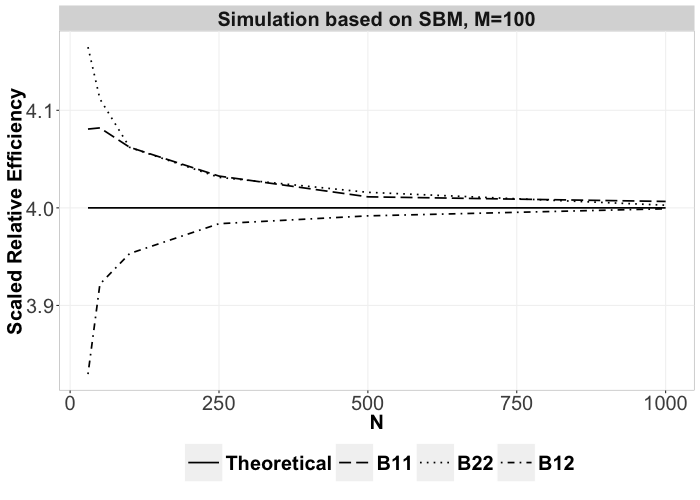
\includegraphics[width=1\textwidth]{RE.png}
	\caption{Scaled relative efficiency in average with different $N$ and fixed $M$ based on 1000 Monte Carlo replicates. Different types of dashed lines denote the simulated scaled RE associated with different blocks. Solid line represents the theoretical value for scaled RE. Observe that $N \cdot \mathrm{RE}_{st}(\bar{A}, \hat{P})$ converges to $1/\rho_s + 1/\rho_t = 4$ as expected.}
	\label{fig:RE}
\end{figure}

To validate that Theorem \ref{thm:ARE} holds with different $\rho$, we fix $N=500$, $M=100$ and run simulations with $\rho_1$ varying from $0.01$ to $0.50$. Figure \ref{fig:RErho} shows $1/\rho_s + 1/\rho_t$, the limit of scaled RE in theory. And the simulated values agree with their corresponding theoretical values perfectly. Notice that when $\rho_1 = 0.5$, the scaled RE has value $4.0$, which agrees with the result in Figure \ref{fig:RE} as expected.

\begin{figure}[!htb]
\centering
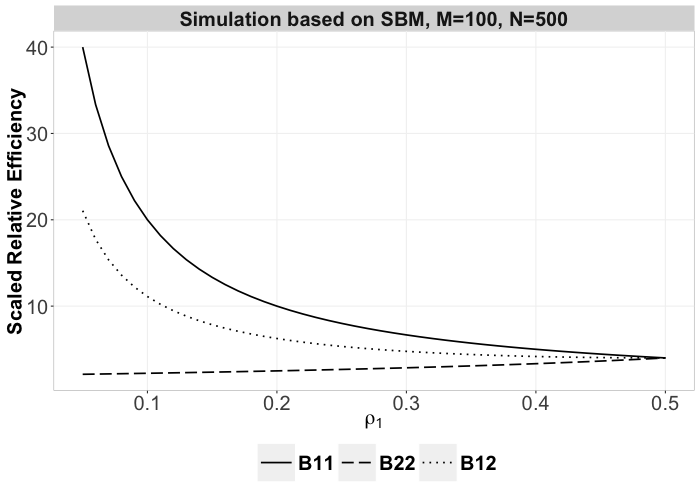
\includegraphics[width=1\textwidth]{Rho.png}
\caption{Simulated results for scaled RE, i.e. $N \cdot \mathrm{RE}_{st}(\bar{A}, \hat{P})$ with $N = 500$ and $M = 100$ of 1000 Monte Carlo replicates while changing $\rho_1$ from 0.1 to 0.9. Scaled relative efficiency in average with different $N$ and fixed $M$ based on 1000 Monte Carlo replicates. Different types of lines denote the simulated values associated with the edges we are averaging over. Notice that when $\rho_1 = 0.5$, the scaled RE has value $4.0$, which agrees with the result in Figure \ref{fig:RE} as expected.}
\label{fig:RErho}
\end{figure}

\subsection{CoRR Brain Graphs: Cross-Validation}

In practice, the graphs may not perfectly follow an RDPG, or even not IEM. But we are still interested in the mean of a collection of graphs. To demonstrate that the estimator $\hat{P}$ is still valid in such cases, we test its performance on DTI data generated with three different atlases (JHU, desikan and CPAC200) available at the Consortium for Reliability and Reproducibility (CoRR) \cite{zuo2014open, gorgolewski2015high}. The dataset contains 454 different brain scans, each of which generates an undirected, unweighted graph with no self-loops. The vertices of the graphs represent different regions in the brain defined by the atlas. For the three atlases we are considering, i.e. JHU, desikan and CPAC200, the number of vertices are 48, 70, 200 respectively. Also, an edge exists between two regions whenever there is at least one white-matter tract connecting the corresponding two parts of the brain. Details of the dataset are provided in Section \ref{section:data}.

By observing 454 graphs generated by the atlas being picked, we use $\hat{P}$ to estimate the mean graph $P$, which is the proportions of the existence of a white-matter tract connecting different parts of the brain. Since $P$ is unknown in practice, we perform a cross-validation study to compare $\bar{A}$ and $\hat{P}$. For each Monte Carlo replicate, we first fix the sample size $M$ and randomly sample $M$ graphs from the total 454 graphs in the dataset. We assure $M$ to be relatively small such that the entry-wise mean of the remaining $(454 - M)$ graphs is a valid approximation of the true probability matrix $P$ we are estimating. Then we can calculate $\bar{A}$ and $\hat{P}$ based on the $M$ samples and compare their performance based on the estimated probability matrix.

We run 1000 simulations on three different atlases with different sample size $M$ and plot the MSE of $\bar{A}$ and $\hat{P}$ in Figure \ref{fig:realdata}. When calculating $\hat{P}$, the dimension $d$ for ASE needs to be selected. For illustrating how the dimension affects the result, we let x-axis to be the dimension $d$ varying from 1 to $N$. Note that this only affects the calculation of $\hat{P}$, that is why the MSE of $\bar{A}$ doesn't change. When $d$ is small, $\hat{P}$ underestimate the dimension and throw away important information, which leads to a relative poor performance. When $d=N$, $\hat{P}$ is equal to $\bar{A}$ since all the information is kept, so that the curve of $\hat{P}$ goes back to $\bar{A}$. In practice, we use algorithms like Zhu and Ghodsi's method or USVT to select the dimension $d$. In the figure, we denote the 3rd elbow of Zhu and Ghodsi by triangle (with largest 95\% confidence interval length to be $3.5$), and denote the USVT with threshold equals 0.7 by square (with largest 95\% confidence interval length to be $0.7$). We can see both algorithms do a good job in dimension selection. When $M$ is small, $\bar{A}$ has large variance which leads to large MSE. Meanwhile, $\hat{P}$ reduces the variance by taking advantages of the graph structure and outperforms $\bar{A}$ with a flexible range of the embedding dimension including what the two algorithms select. With a relatively large $M$, $\bar{A}$ has information to provide a good enough estimation, leaving less space for improvement. As a result, both estimators perform almost perfect when $M$ is large.

\begin{figure}[!htb]
\centering
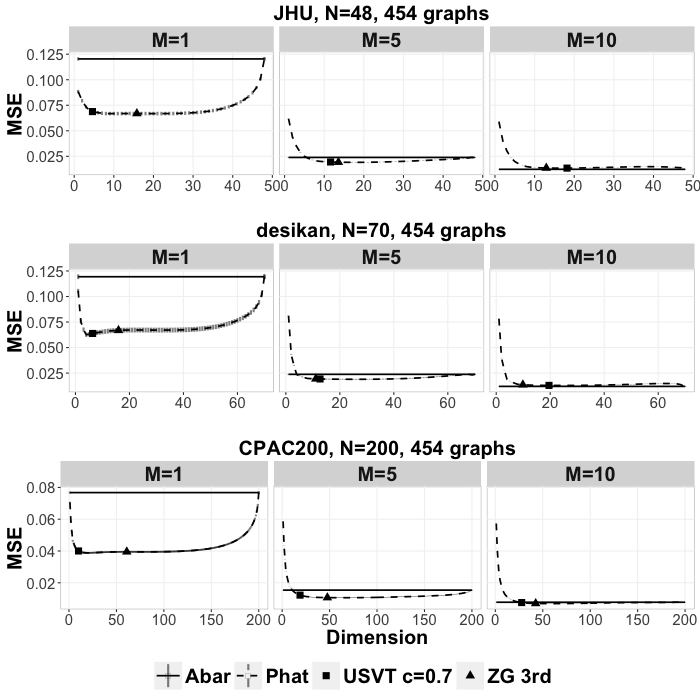
\includegraphics[width=1\textwidth]{realdata.png}
\caption{Comparison of MSE between $\bar{A}$ (solid line) and $\hat{P}$ (dashed line) for three dataset (JHU, desikan and CPAC200) while embedding the graphs into different dimensions with different size $M$ of the subsamples. The dimension chosen by the 3rd elbow of Zhu and Ghodsi is denoted in triangle (with largest 95\% confidence interval length to be $3.5$), and chosen by USVT with threshold equals 0.7 is denoted in square (with largest 95\% confidence interval length to be $0.7$).  Vertical intervals represent the 95\% confidence interval.  When $M$ is small, $\hat{P}$ outperforms $\bar{A}$ with a flexible range of the embedding dimension including what Zhu and Ghodsi selects.}
\label{fig:realdata}
\end{figure}

For illustration, we randomly take one sample of size $M=5$ based on desikan atlas, and then calculate $\bar{A}$ and $\hat{P}$. The dimension Zhu and Ghodsi's 3rd elbow select is $d=11$. In Figure \ref{fig:Matrix_desikan_m5}, the estimates $\bar{A}$ and $\hat{P}$ as well as the sample mean of 454 graphs (as a close estimate of $P$) are plotted. Since the sample size is small, there are a lot of pairs of vertices with no edges in the 5 observations leading to white spots in $\bar{A}$, especially when the corresponding proportion of the existence of an edge is small. This is compensated in $\hat{P}$ by taking the graph structure into account. In the figure, we see $\hat{P}$ has fewer white spots and look much similar to $P$ compared to $\bar{A}$. Moreover, Figure \ref{fig:Diff_desikan_m5} shows the heat plot of the absolute estimation error $|\bar{A} - P|$ and $|\hat{P}-P|$ respectively. The lower triangular matrix shows the actual absolute difference while the upper triangular matrix only highlights the edges with absolute differences larger than 0.4. There are 18 edges from $\bar{A}$ and 6 edges from $\hat{P}$ being highlighted in the figure, indicating the better performance of $\hat{P}$.

There are lots of places that $\hat{P}$ is better from Figure \ref{fig:Matrix_desikan_m5} and Figure \ref{fig:Diff_desikan_m5} as mentioned above. Here are the actual places in the brain that $\hat{P}$ is better. In Figure \ref{fig:Diff_between_desikan}, we plot the top 5 regions of the brain and top 50 connections between regions with the largest difference $|\bar{A} - P| - |\hat{P} - P|$. Red edges indicate that $\hat{P}$ overestimate $P$ while blue means that $\hat{P}$ underestimate $P$. The edge width is determined by the estimation error. Connections with larger estimation error are represented by thicker lines. This figure shows the regions and connections of the brain where $\hat{P}$ outperforms $\bar{A}$ the most for estimating $P$.

The result demonstrates that $\hat{P}$ gives a better estimate than $\bar{A}$ based on the CoRR dataset with three atlases. 
More importantly, this improvement is insensitive to the embedding dimension we choose as long as we don't underestimate it, which makes our estimator more robust and useful in analyzing real data.

\begin{figure}[!htb]
\centering
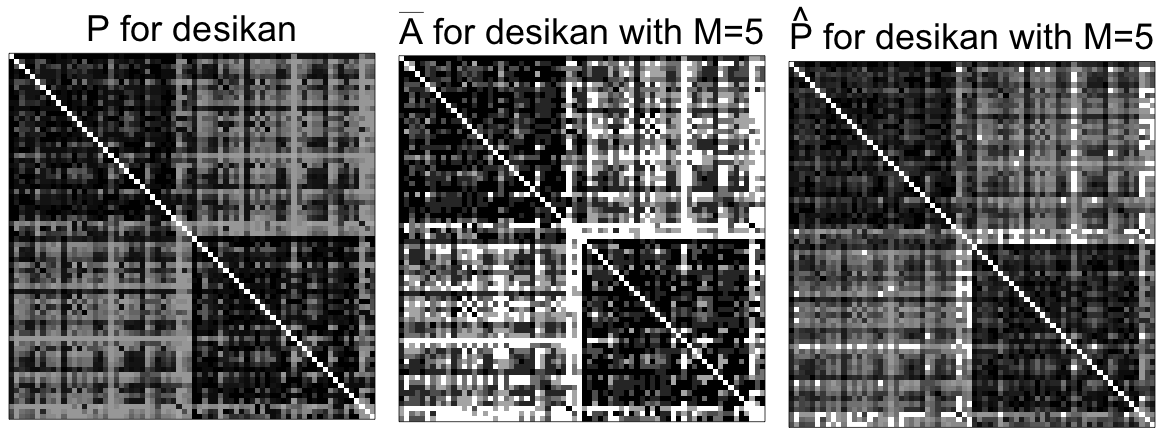
\includegraphics[width=1\textwidth]{Matrix_desikan_m5.png}
\caption{Comparison between the mean of 454 graphs $P$ and two estimates $\bar{A}$ and $\hat{P}$ derived from a sample of size $M=5$ from desikan dataset while embedding the graphs into dimension $d=11$ selected by the 3rd elbow of ZG method. From the figure, we can see that $\hat{P}$ is a better estimation of $P$ than $\bar{A}$.}
\label{fig:Matrix_desikan_m5}
\end{figure}

\begin{figure}
\centering
\begin{subfigure}{.5\textwidth}
  \centering
  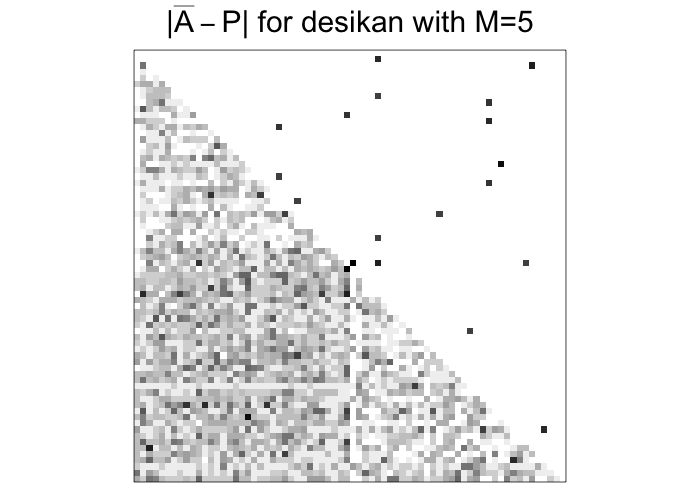
\includegraphics[width=1.2\linewidth]{Diff2_desikan_m5.png}
\end{subfigure}%
\begin{subfigure}{.5\textwidth}
  \centering
  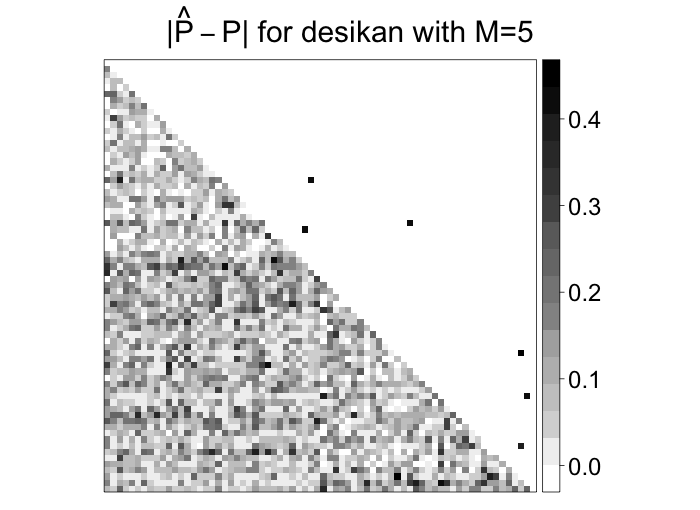
\includegraphics[width=1.2\linewidth]{Diff3_desikan_m5.png}
\end{subfigure}
\caption{Heat plot of the absolute estimation error $|\bar{A} - P|$ and $|\hat{P} - P|$ for a sample of size $M=5$ from desikan dataset while embedding the graphs into dimension $d=11$ selected by the 3rd elbow of ZG method. The lower triangular matrix shows the actual absolute difference, while the upper triangular matrix only highlights the edges with absolute differences larger than $0.4$. The fact that 18 edges from $\bar{A}$ and 6 edges from $\hat{P}$ being highlighted shows the better performance of $\hat{P}$.}
\label{fig:Diff_desikan_m5}
\end{figure}

\begin{figure}[!htb]
\centering
\includegraphics[width=1\textwidth]{Diff_between_desikan.png}
\caption{Top 5 regions of the brain (vertices in graphs) and top 50 connections between regions (edges in graphs) with largest difference $|\bar{A} - P| - |\hat{P} - P|$. Red edges indicate that $\hat{P}$ overestimate $P$ while blue means that $\hat{P}$ underestimate $P$. The edge width is determined by the estimation error. Connections with larger estimation error are represented by thicker lines. This figure shows the regions and connections of the brain where $\hat{P}$ outperforms $\bar{A}$ the most for estimating $P$.}
\label{fig:Diff_between_desikan}
\end{figure}


%\begin{figure}[!htb]
%\centering
%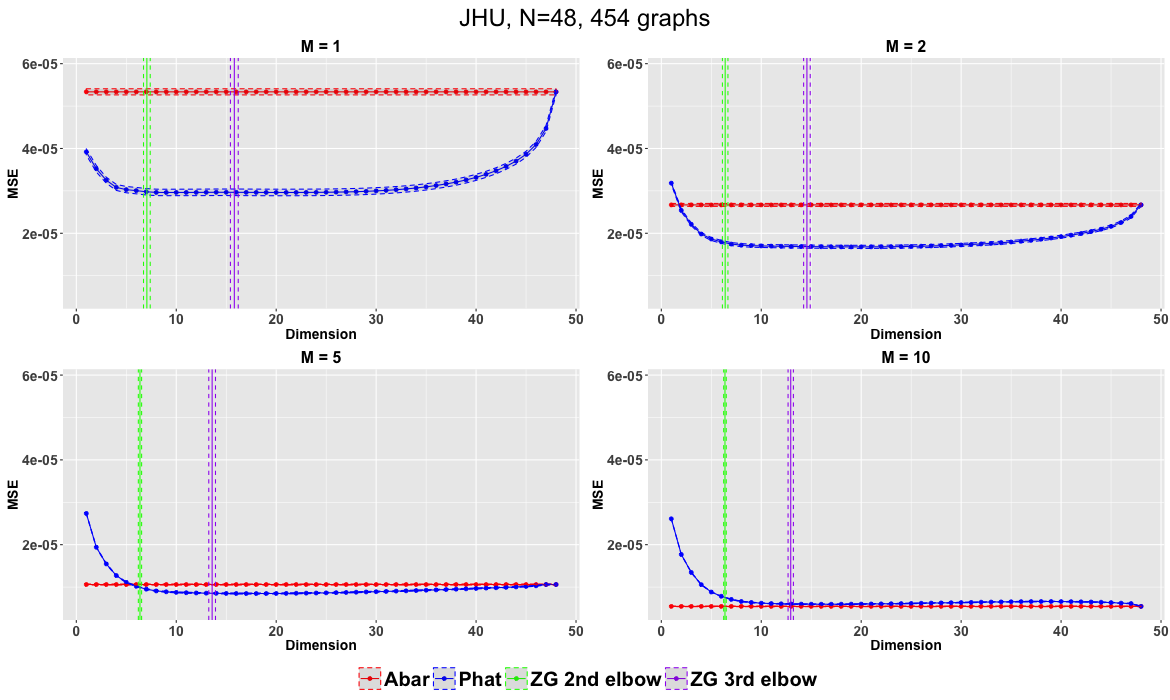
\includegraphics[width=1\textwidth]{JHU.png}
%\caption{Comparison of MSE between $\bar{A}$ (solid line) and $\hat{P}$ (dashed line) for JHU dataset while embedding the graphs into different dimensions with different size $M$ of the subsamples. The dimension chosen by the 3rd elbow of Zhu and Ghodsi is denoted in triangle, and chosen by USVT with threshold equals 0.7 is denoted in square. Vertical intervals represent the 95\% confidence interval. When $M$ is small, $\hat{P}$ outperforms $\bar{A}$ with a flexible range of the embedding dimension including what Zhu and Ghodsi selects.}
%\label{fig:JHU}
%\end{figure}
%
%\begin{figure}[!htb]
%\centering
%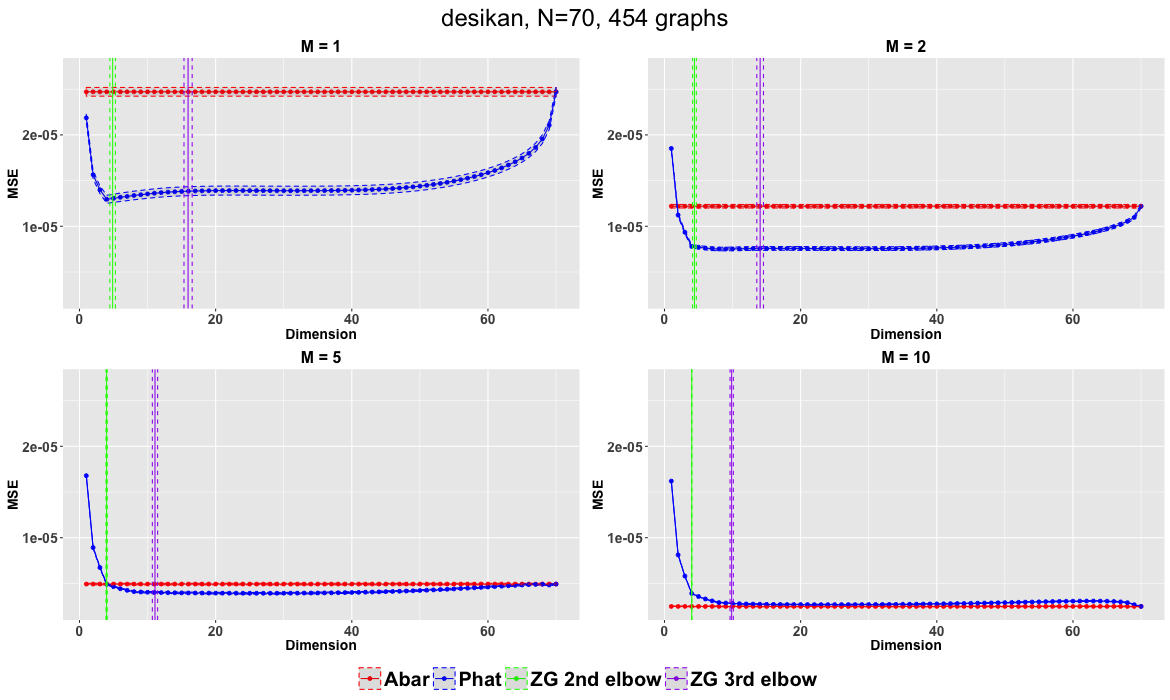
\includegraphics[width=1\textwidth]{desikan.png}
%\caption{Comparison of MSE between $\bar{A}$ (solid line) and $\hat{P}$ (dashed line) for desikan dataset while embedding the graphs into different dimensions with different size $M$ of the subsamples. The dimension chosen by the 3rd elbow of Zhu and Ghodsi is denoted in triangle, and chosen by USVT with threshold equals 0.7 is denoted in square.  Vertical intervals represent the 95\% confidence interval.  When $M$ is small, $\hat{P}$ outperforms $\bar{A}$ with a flexible range of the embedding dimension including what Zhu and Ghodsi selects.}
%\label{fig:desikan}
%\end{figure}
%
%\begin{figure}[!htb]
%\centering
%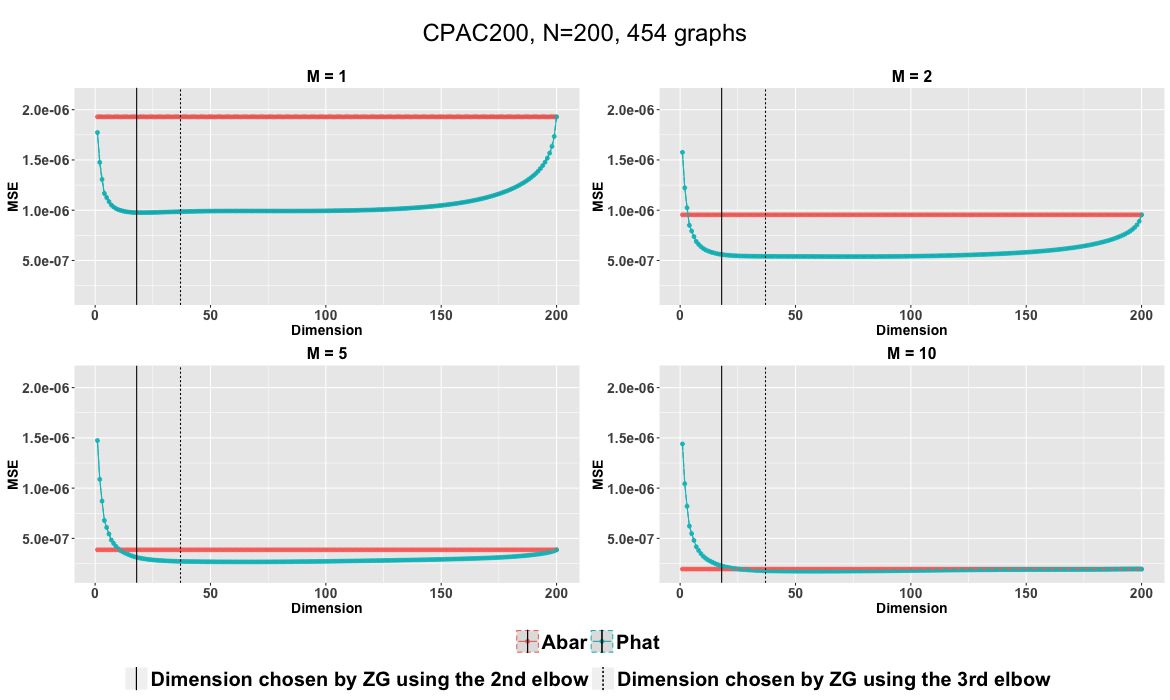
\includegraphics[width=1\textwidth]{CPAC200.png}
%\caption{Comparison of MSE between $\bar{A}$ (solid line) and $\hat{P}$ (dashed line) for CPAC200 dataset while embedding the graphs into different dimensions with different size $M$ of the subsamples. The dimension chosen by the 3rd elbow of Zhu and Ghodsi is denoted in triangle, and chosen by USVT with threshold equals 0.7 is denoted in square.  Vertical intervals represent the 95\% confidence interval.  When $M$ is small, $\hat{P}$ outperforms $\bar{A}$ with a flexible range of the embedding dimension including what Zhu and Ghodsi selects.}
%\label{fig:CPAC200}
%\end{figure}
%
%\begin{figure}
%\centering
%\begin{subfigure}{.33\textwidth}
%  \centering
%  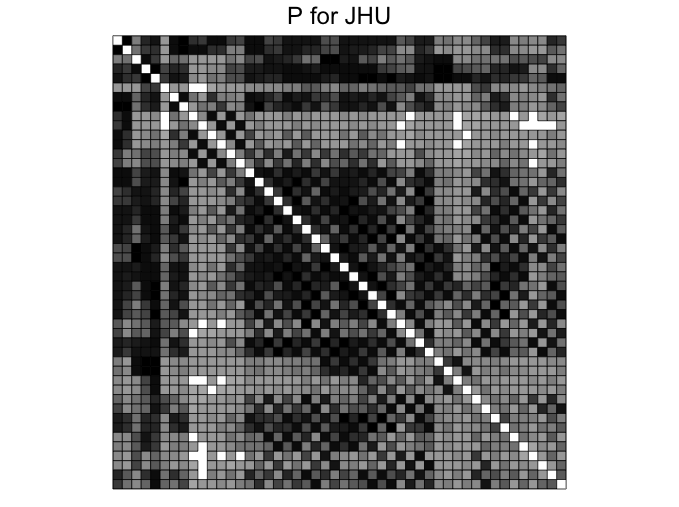
\includegraphics[width=1.2\linewidth]{P_JHU.png}
%\end{subfigure}%
%\begin{subfigure}{.33\textwidth}
%  \centering
%  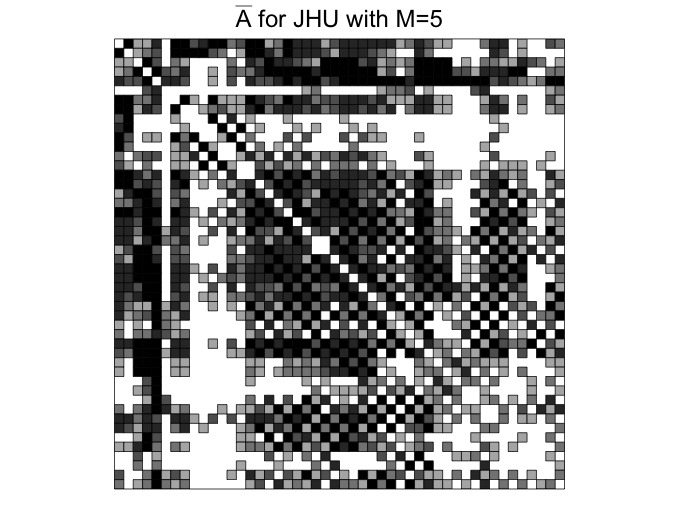
\includegraphics[width=1.2\linewidth]{Abar_JHU_m5.png}
%\end{subfigure}
%\begin{subfigure}{.33\textwidth}
%  \centering
%  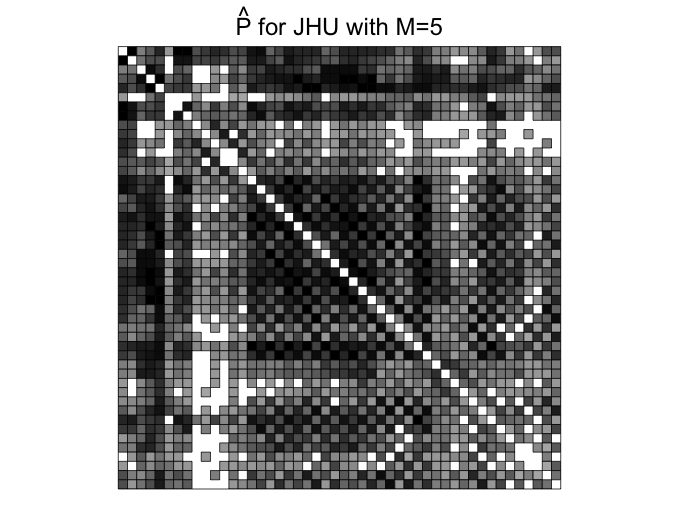
\includegraphics[width=1.2\linewidth]{Phat_JHU_m5.png}
%\end{subfigure}
%\caption{Comparison between the mean of 454 graphs $P$ and two estimates $\bar{A}$ and $\hat{P}$ derived from a sample of size $M=5$ from JHU dataset while embedding the graphs into dimension $d=15$ selected by the 3rd elbow of ZG method.}
%\label{fig:adj_JHU_m5}
%\end{figure}
%
%\begin{figure}[!htb]
%\centering
%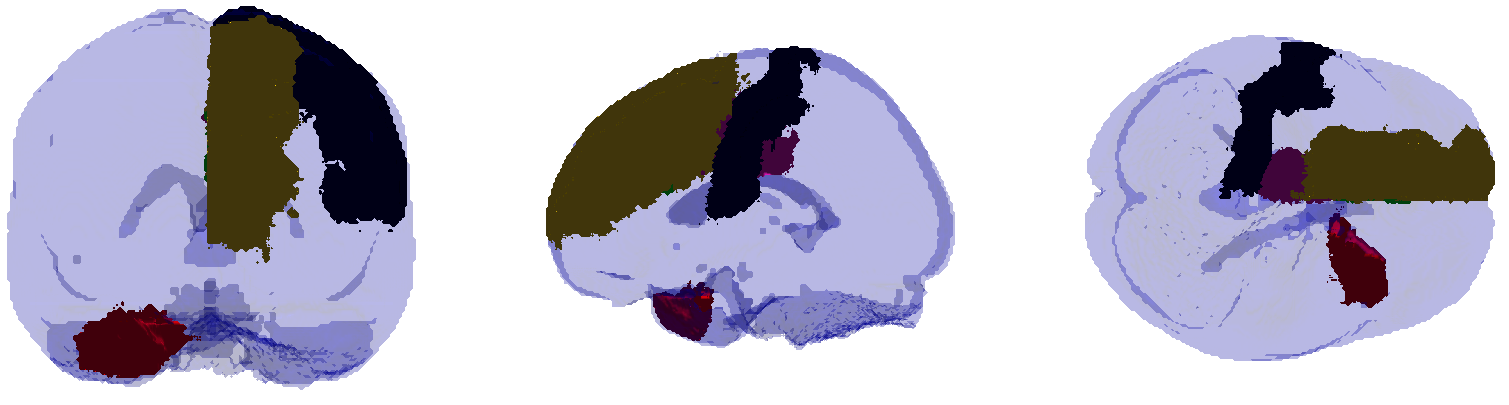
\includegraphics[width=1\textwidth]{Vertex_Diff_Phat_desikan.png}
%\caption{Top 5 regions of the brain (vertices in graphs) with largest absolute difference $|\hat{P} - P|$.}
%\label{fig:Vertex_Diff_Phat_desikan}
%\end{figure}
%
%\begin{figure}[!htb]
%\centering
%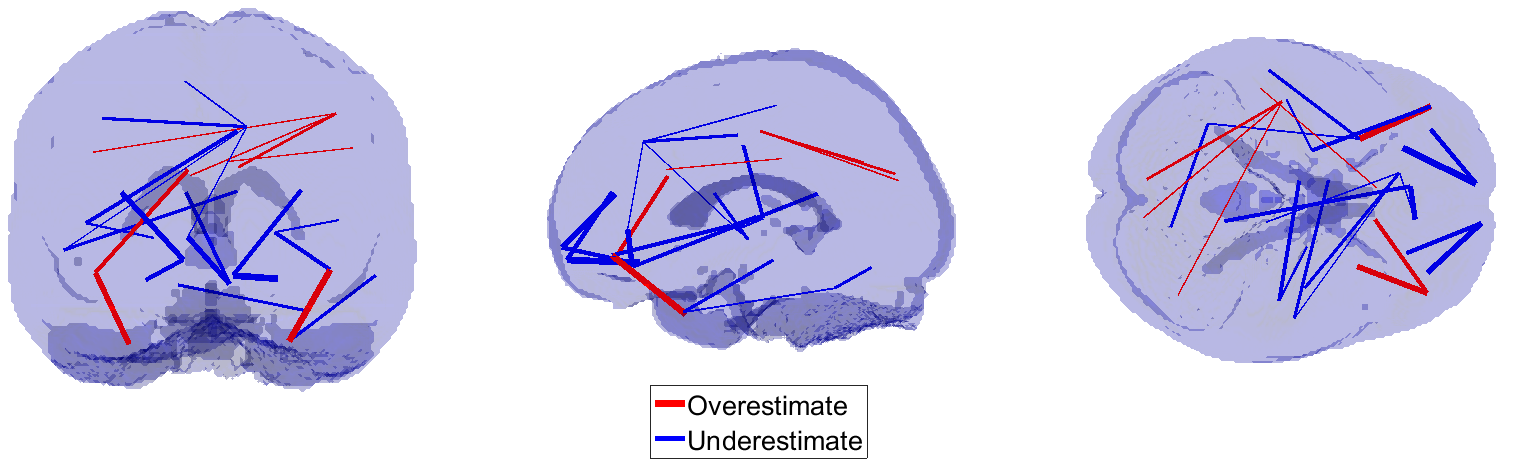
\includegraphics[width=1\textwidth]{Edge_Diff_Phat_desikan.png}
%\caption{Top 1\% (49) connections between regions (edges in graphs) with largest absolute difference $|\hat{P} - P|$.}
%\label{fig:Vertex_Diff_Phat_desikan}
%\end{figure}


\subsection{Simulation under the Full Rank Independent Edge Model}

While the theory we have is based on the low rank assumption implied by the RDPG, $\hat{P}$ sometimes wins the bias-variance tradeoff even when the graphs have full rank structure. To illustrate this point, instead of the low rank SBM, we run simulations under the full rank independent edge model with the probability matrix $P$, defined as the sample mean of the 454 graphs in the desikan dataset.

Figure \ref{fig:sim_desikan} compare the MSE between $\bar{A}$ (solid line) and $\hat{P}$ (dashed line) for simulated data based on the full rank probability matrix $P$ as the sample mean in desikan dataset while embedding the graphs into different dimensions with different size $M$ of the subsamples. Vertical intervals represent the 95\% confidence interval. We see similar results as in the SBM setting. When $M$ is small, $\hat{P}$ outperforms $\bar{A}$ with a flexible range of the embedding dimension including what Zhu and Ghodsi selects. When $M$ is large enough, both estimators perform almost perfect.

So $\hat{P}$ does a good job even when the low rank assumption of the model is violated. This simulation shows again the robustness of $\hat{P}$.


\begin{figure}[!htb]
\centering
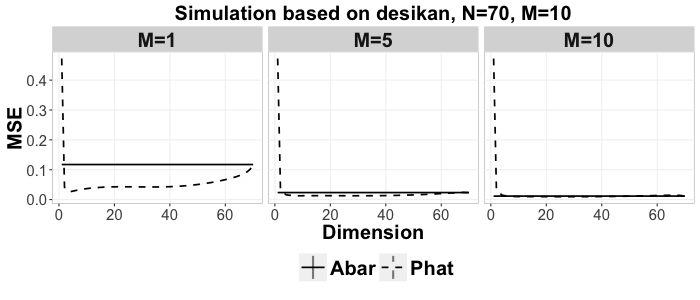
\includegraphics[width=1\textwidth]{sim_desikan.png}
\caption{Comparison of MSE between $\bar{A}$ (solid line) and $\hat{P}$ (dashed line) for simulated data based on the full rank probability matrix $P$ as the sample mean in desikan dataset while embedding the graphs into different dimensions with different size $M$ of the subsamples. Vertical intervals represent the 95\% confidence interval. When $M$ is small, $\hat{P}$ outperforms $\bar{A}$ with a flexible range of the embedding dimension including what Zhu and Ghodsi selects.}
\label{fig:sim_desikan}
\end{figure}



\section{Discussion}

\subsection{Summary}
In this paper, we propose a better way to estimate the mean of a collection of graphs.Motivated by RDPG, our methodology take advantage of the low-rank structure of the graphs by applying ASE to the entry-wise MLE. We then give a closed form for the asymptotical relative efficiency between the entry-wise MLE $\bar{A}$ and our estimator $\hat{P}$, which theoretically proves that $\hat{P}$ has smaller MSE when $N$ is sufficiently large. These results are demonstrate by various simulations. Moreover, our estimator also outperforms the entry-wise MLE in the CoRR brain graphs and in the full-rank simulation, which shows that $\hat{P}$ still performs well even when the low-rank assumption is violated. It demonstrate that $\hat{P}$ is robust and can be applied in practice.


\subsection{Future Work}
In this paper, we assume that the adjacency matrix is observed without contamination. However, generally there will be noise in practice. With contaminations, robust estimators like ML$q$E is preferred. If an estimator can not only inherit robustness from the robust estimators but also has small variance by taking advantage of the low rank structure of the graphs, it will be very useful.

Meanwhile, estimating the rank of the graph structure accurately will certainly help improve the performance of the estimator $\hat{P}$. Now we are using Zhu and Ghodsi's method and USVT, but there is still a lot of space for improvement, especially in this particular case.







\section{Methods}

\subsection{Choosing Dimension}
\label{section:dim_select}
Often in dimensionality reduction techniques, the choice for dimension $d$, relies on visually analyzing a plot of the ordered eigenvalues, looking for a ``gap'' or ``elbow'' in the scree-plot. Zhu and Ghodsi \cite{zhu2006automatic} present an automated method for finding this gap in the scree-plot that takes only the ordered eigenvalues as an input. In order to prevent underestimating $d$, which is much more harmful than overestimating, we use the 3rd elbow in the experiments performed in this work.

Universal Singular Value Thresholding (USVT) \cite{chatterjee2015matrix} is a simple estimation procedure proposed by Chatterjee that works for any matrix that has ``a little bit of structure''. Basically in our setting, it selects the dimension $d$ as the number singular values that are greater than a constant $c$ times $\sqrt{N/M}$. In the simulation, we set $c = 0.7$.



\subsection{Graph Diagonal Augmentation}
\label{section:diag_aug}
The graphs examined in this work are hollow, in that there are no self-loops and thus the diagonal entries of the adjacency matrix are 0. This leads to a bias in the calculation of the eigenvectors. To compensate such bias, we use an iterative method developed by Scheinerman and Tucker \cite{scheinerman2010modeling} to augment the diagonal before ASE. In the experiments, we are using 1 iteration of Scheinerman's method to do the diagonal augmentation.



\subsection{Dataset Description}
\label{section:data}
The original dataset is from the Emotion and Creativity One Year Retest Dataset provided by Qiu, Zhang and Wei from Southwest University available at the Consortium for Reliability and Reproducibility (CoRR) \cite{zuo2014open, gorgolewski2015high}. It is comprised of 235 subjects, all of whom were college students. Each subject underwent two sessions of anatomical, resting state DTI scans, spaced one year apart. Due to the incomplete data, the true number of scans is 454.

When deriving MR connectomes, the NeuroData team parcellate the brain into groups of nodes as defined by anatomical atlases \cite{neurodata, kiar2016graph}. The atlases are defined either physiologically or structurally by neuroanatomists (Desikan and JHU), or are generated using a segmentation algorithm looking for certain features or groupings (CPAC200).

The graphs we are using are processed by NeuroData team from DTI data of the original dataset generated with different atlases (desikan, JHU and CPAC200), each containing different region/node definitions. The graphs are undirected, unweighted and with no self-loops. An edge exists between two regions when there is at least one white-matter tract connecting the corresponding two parts of the brain.


\subsection{Outline for the Proof of the Theorems}
\label{section:outline_proof}
Here we provide an outline of the proof for the MSE($\hat{P}$) result presented in Section \ref{section:theoretical_result}.
	
When comparing two estimators, the first thing we need to consider is consistency.
It is easy to see that $\bar{A}$ is unbiased as an estimate of $P$. Moreover, since two latent positions are conditionally asymptotically independent by extended version of Theorem 1 in Athreya et al. (2013) \cite{athreya2013limit}, we know $\hat{P}$ is consistent, as well as $\bar{A}$.

Thus the relative efficiency between $\hat{P}$ and $\bar{A}$, which is equivalent to the ratio of mean square errors in this case, is a good indicate in comparison.

Since $\hat{P}_{ij} = \hat{X}_i^T \hat{X}_j$ is a noisy version of the dot product of $\nu_s^T \nu_t$, by Equation 5 in Brown and Rutemiller (1977) \cite{brown1977means}, combined with asymptotic independence between $\hat{X}_i$ and $\hat{X}_j$, and the covariance matrices given by extended version of Theorem 1 in Athreya et al. (2013) \cite{athreya2013limit}, we have the variance of $\hat{P}_{ij}$ converges to $\left( 1/\rho_{\tau_i} + 1/\rho_{\tau_j} \right) P_{ij} (1-P_{ij})/(N \cdot M)$ as $N \rightarrow \infty$. Since the variance of $\bar{A}_{ij}$ is $P_{ij} (1-P_{ij})/M$, the relative efficiency between $\hat{P}_{ij}$ and $\bar{A}_{ij}$ is approximately $(\rho_{\tau_i}^{-1} + \rho_{\tau_j}^{-1})/N$ when $N$ is sufficiently large.
	
The (relative) full proof is provided here: \\
https://www.overleaf.com/2776898cydwhv. Feel free to edit it.

\bibliography{Bib}{}
\bibliographystyle{plain}


\end{document}